\section{Introducción a la programación estructurada.}
\setcounter{subsection}{3}

\subsection{Repaso}

\begin{minipage}{0.5\textwidth}
  \textbf{si} \it{condición} \textbf{entonces}\\
  \hspace*{10mm}\it{proceso}\\
  \textbf{fin si}\\
\end{minipage}
\begin{minipage}{0.5\textwidth}
\center
  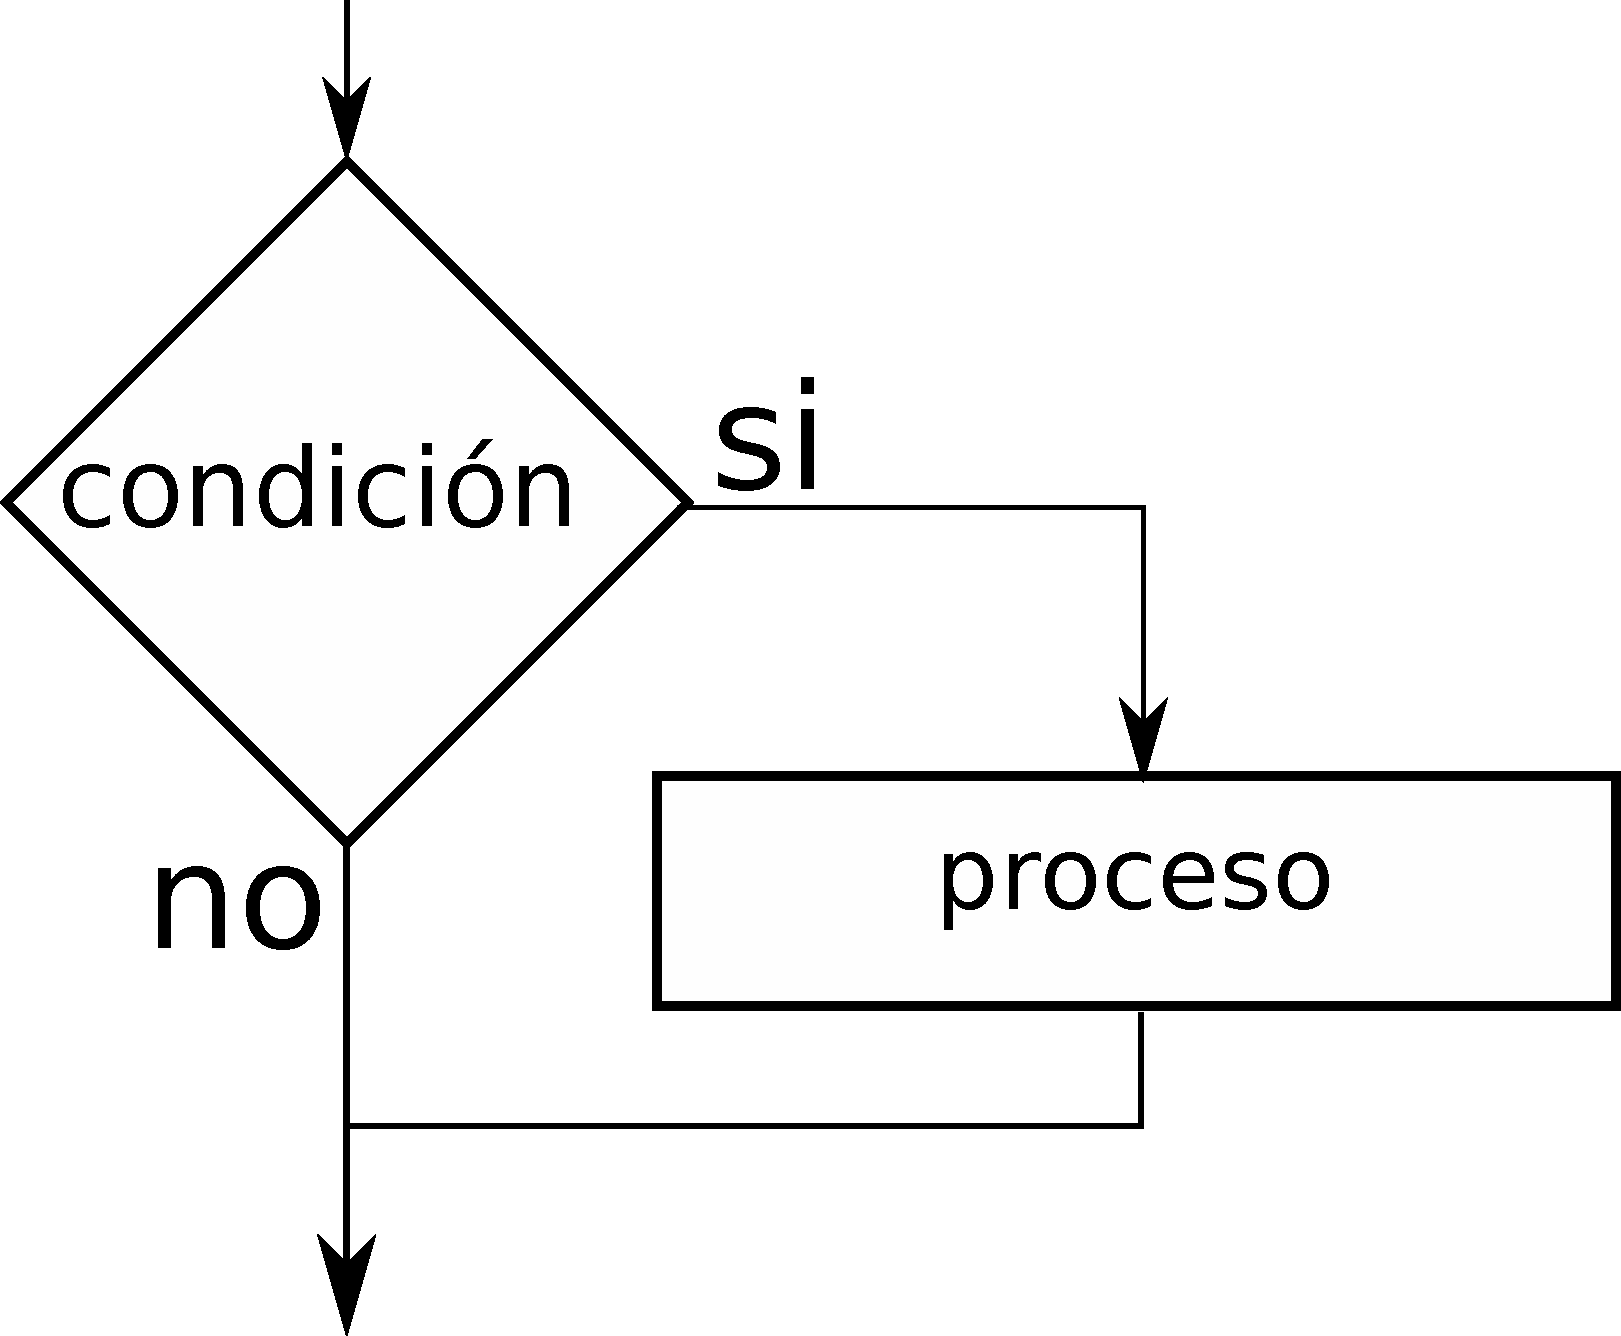
\includegraphics[height=40mm]{img/if.pdf}
\end{minipage}

\vspace{10mm}

\begin{minipage}{0.5\textwidth}
  \textbf{si} \it{condición} \textbf{entonces}\\
  \hspace*{10mm}\it{proceso 1}\\
  \textbf{si no}\\
  \hspace*{10mm}\it{proceso 2}\\
  \textbf{fin si}\\
\end{minipage}
\begin{minipage}{0.5\textwidth}
  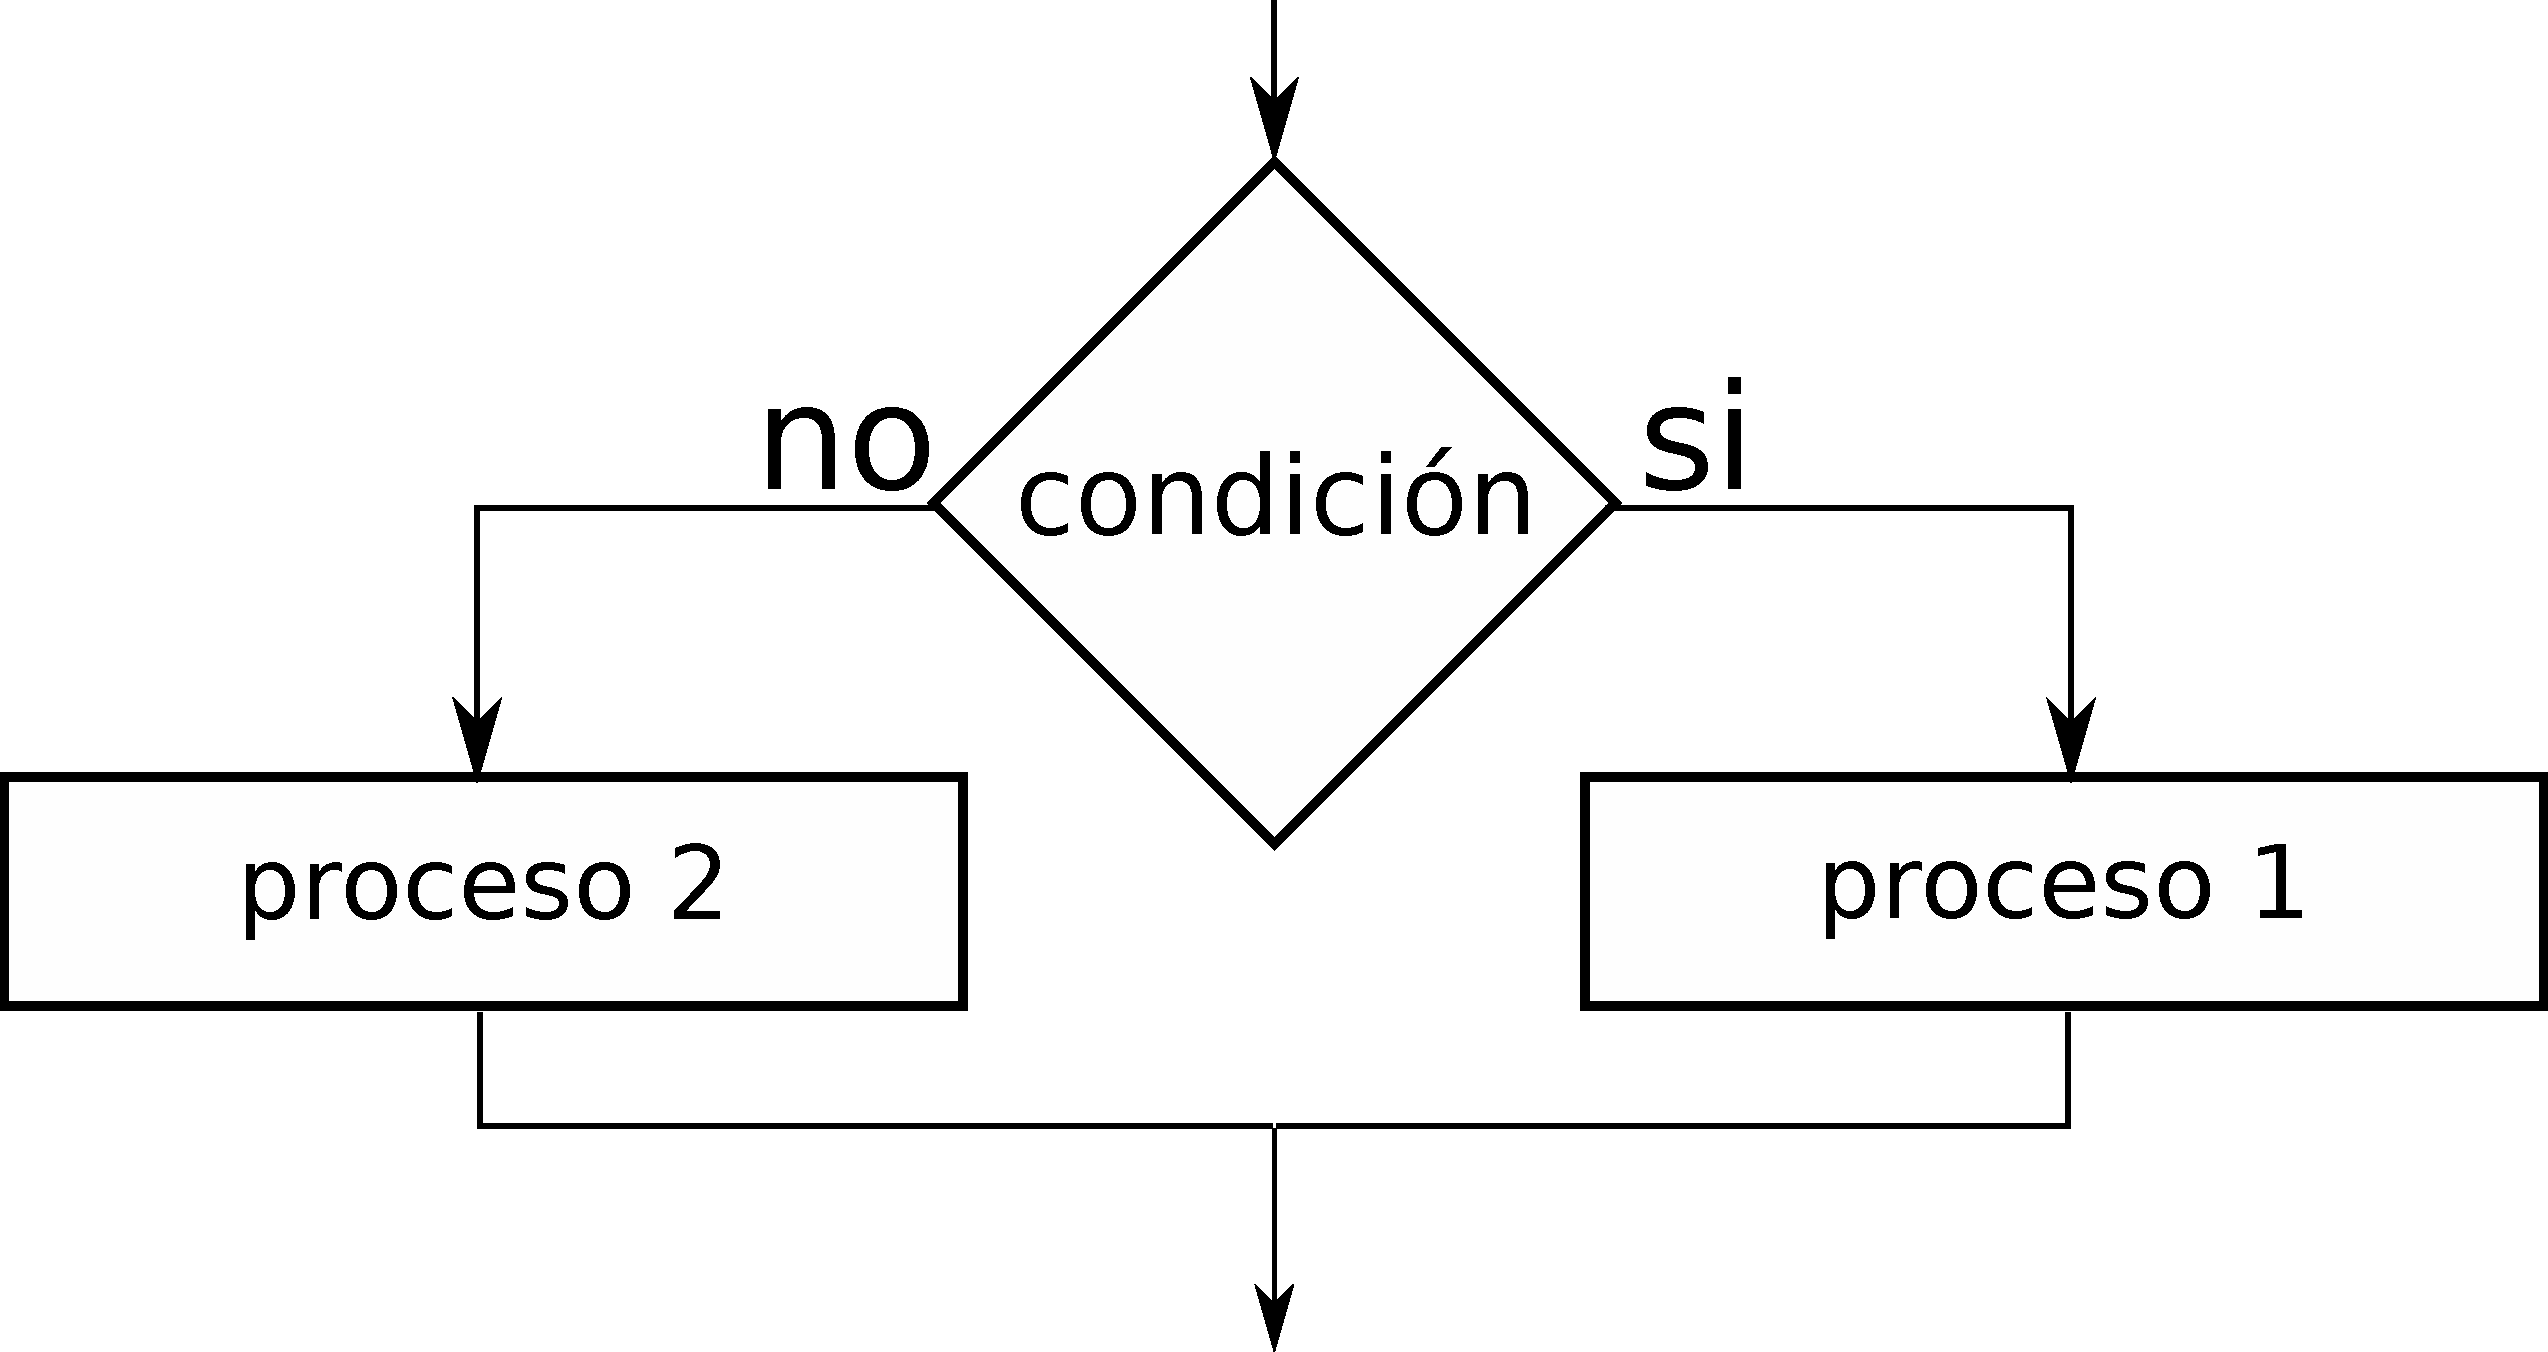
\includegraphics[height=40mm]{img/if_else.pdf}
\end{minipage}

\vspace{10mm}

\begin{minipage}{0.5\textwidth}
  \textbf{mientras} \it{condición} \\
  \hspace*{10mm}\it{proceso}\\
  \textbf{fin mientras}\\
\end{minipage}
\begin{minipage}{0.5\textwidth}
\center
  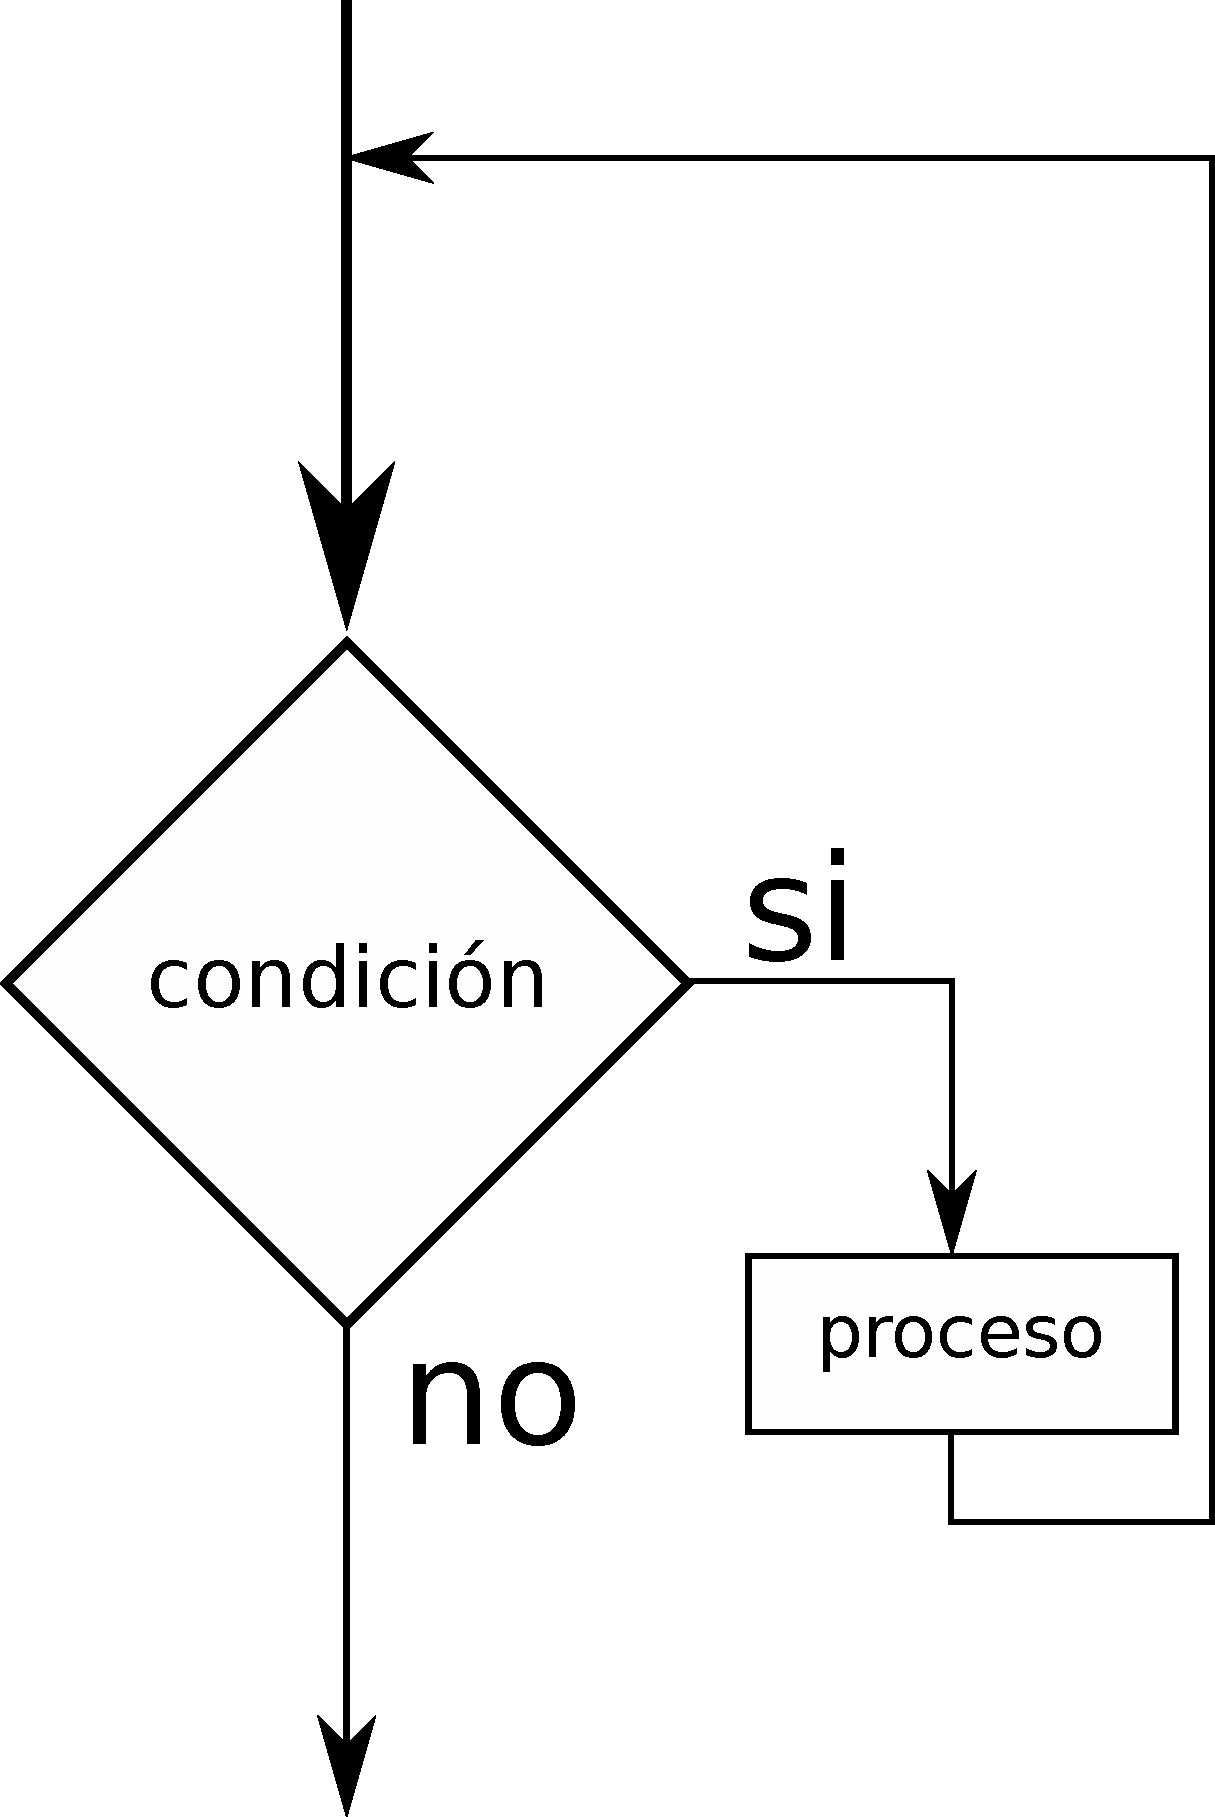
\includegraphics[height=40mm]{img/mientras.pdf}
\end{minipage}

\vspace{10mm}

\begin{minipage}{0.5\textwidth}
  \textbf{hacer} \\
  \hspace*{10mm}\it{proceso}\\
  \textbf{mientras} \it{condición}\\
\end{minipage}
\begin{minipage}{0.5\textwidth}
\center
  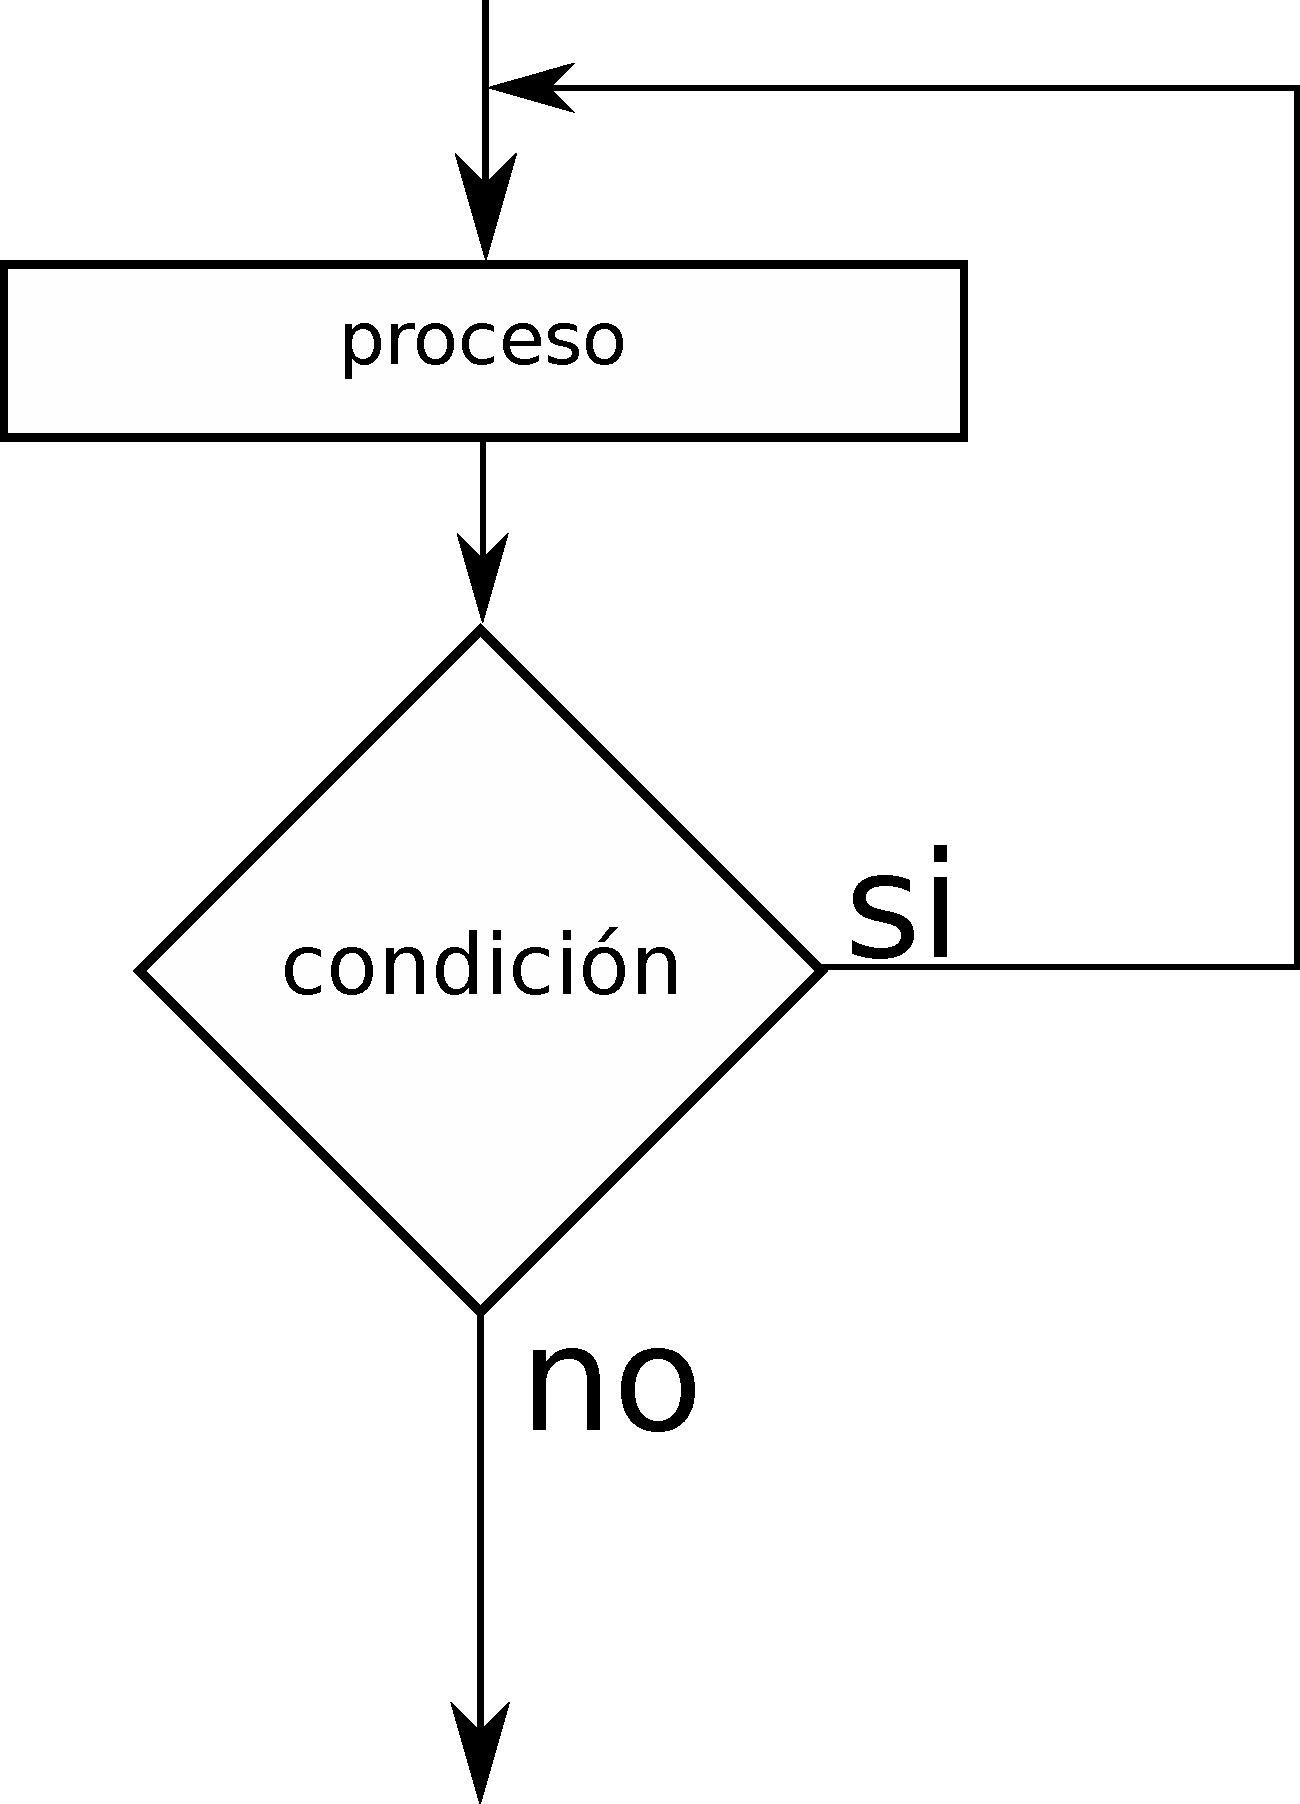
\includegraphics[height=40mm]{img/hacer_mientras.pdf}
\end{minipage}

% \setcounter{subsection}{4}
\subsubsection{Ejercicio}
Realizar un programa que solicite la dimensión en cm de lados de un rectángulo y muestre la superficie del mismo

\subsubsection*{Solución}
\begin{lstlisting}[style=pseudocodigo]
imprimir: Ingrese la longitud del primer lado
leer:lado1
imprimir: Ingrese la longitud del segundo lado
leer: lado2
superficie = lado1 * lado2
imprimir: superficie
\end{lstlisting}

\begin{figure}[h!]
  \centering
  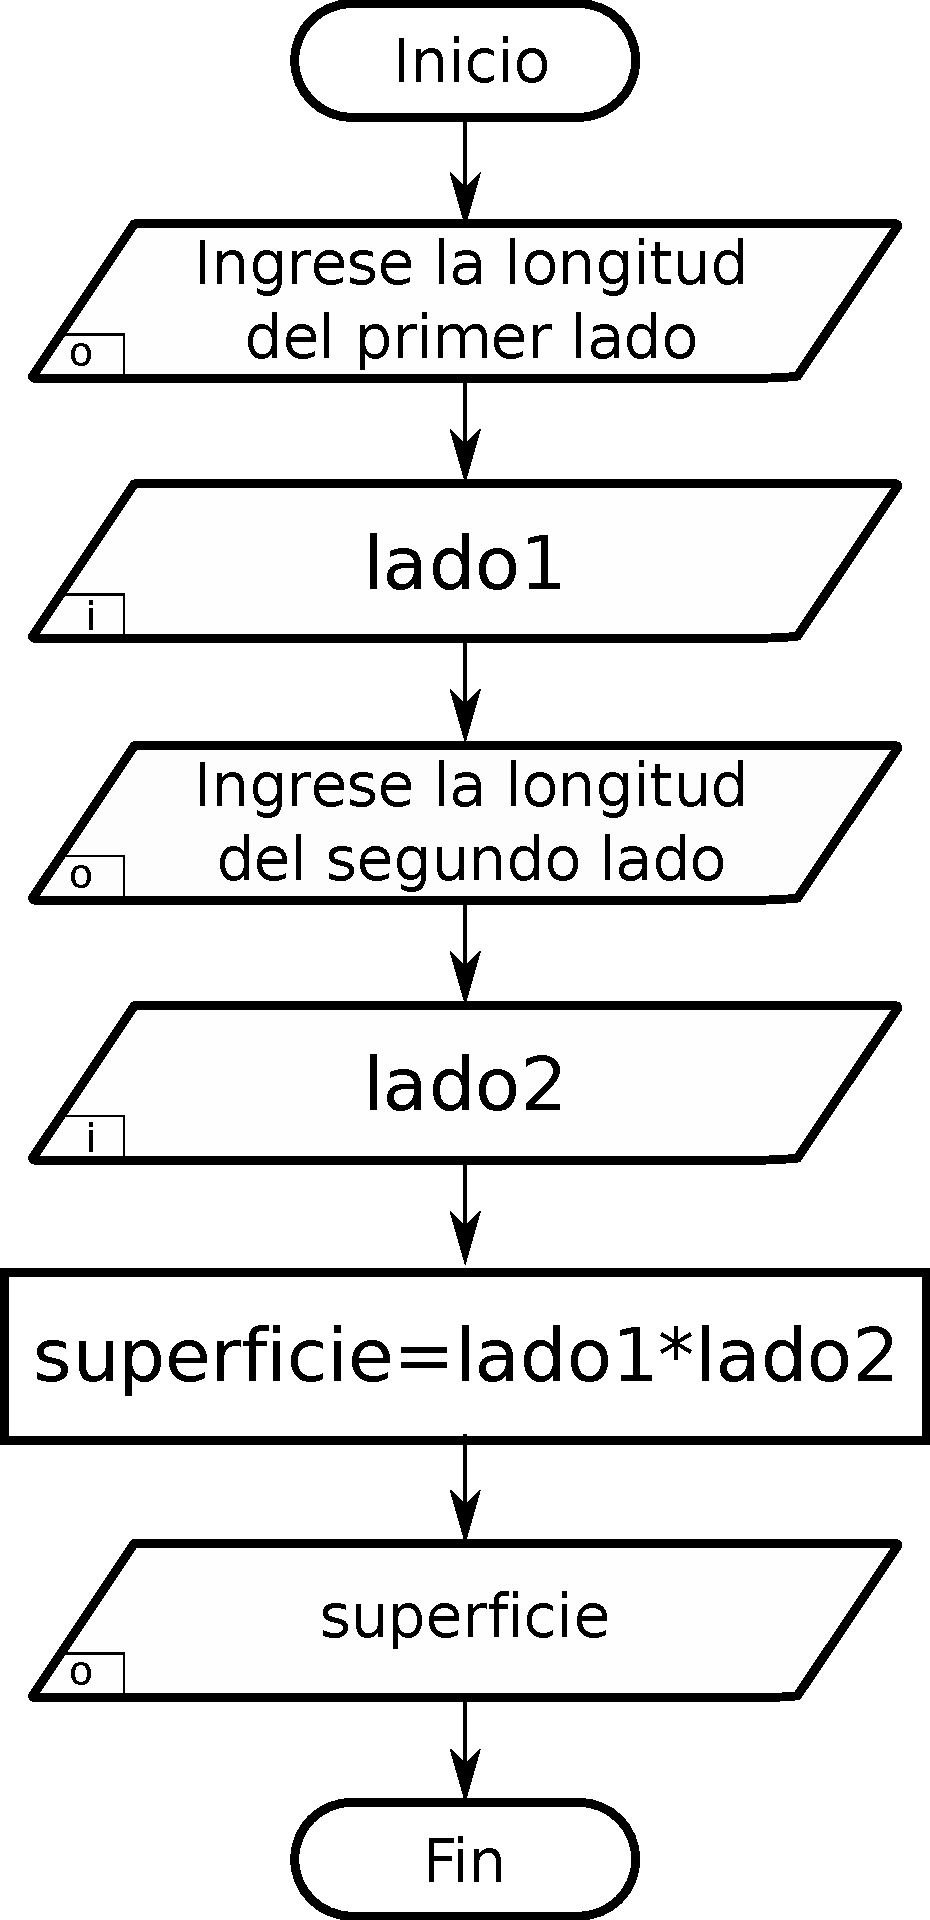
\includegraphics[height=80mm]{./img/ejercicio_1.pdf} 
\end{figure}

\pagebreak

\subsubsection{Ejercicio}
Escribir un algoritmo que solicite la edad de dos hermanos, muestre un mensaje indicando el mayor y su diferencia.

\subsubsection*{Solución}
\begin{lstlisting}[style=pseudocodigo]
imprimir: Ingrese la primera edad
leer:edad1
imprimir: Ingrese la segunda edad
leer: edad2
si edad1 > edad2 entonces
  imprimir: El primero es el mayor
si no
  imprimir: El segundo es el mayor
imprimir: diferencia
\end{lstlisting}

\begin{figure}[h!]
  \centering
  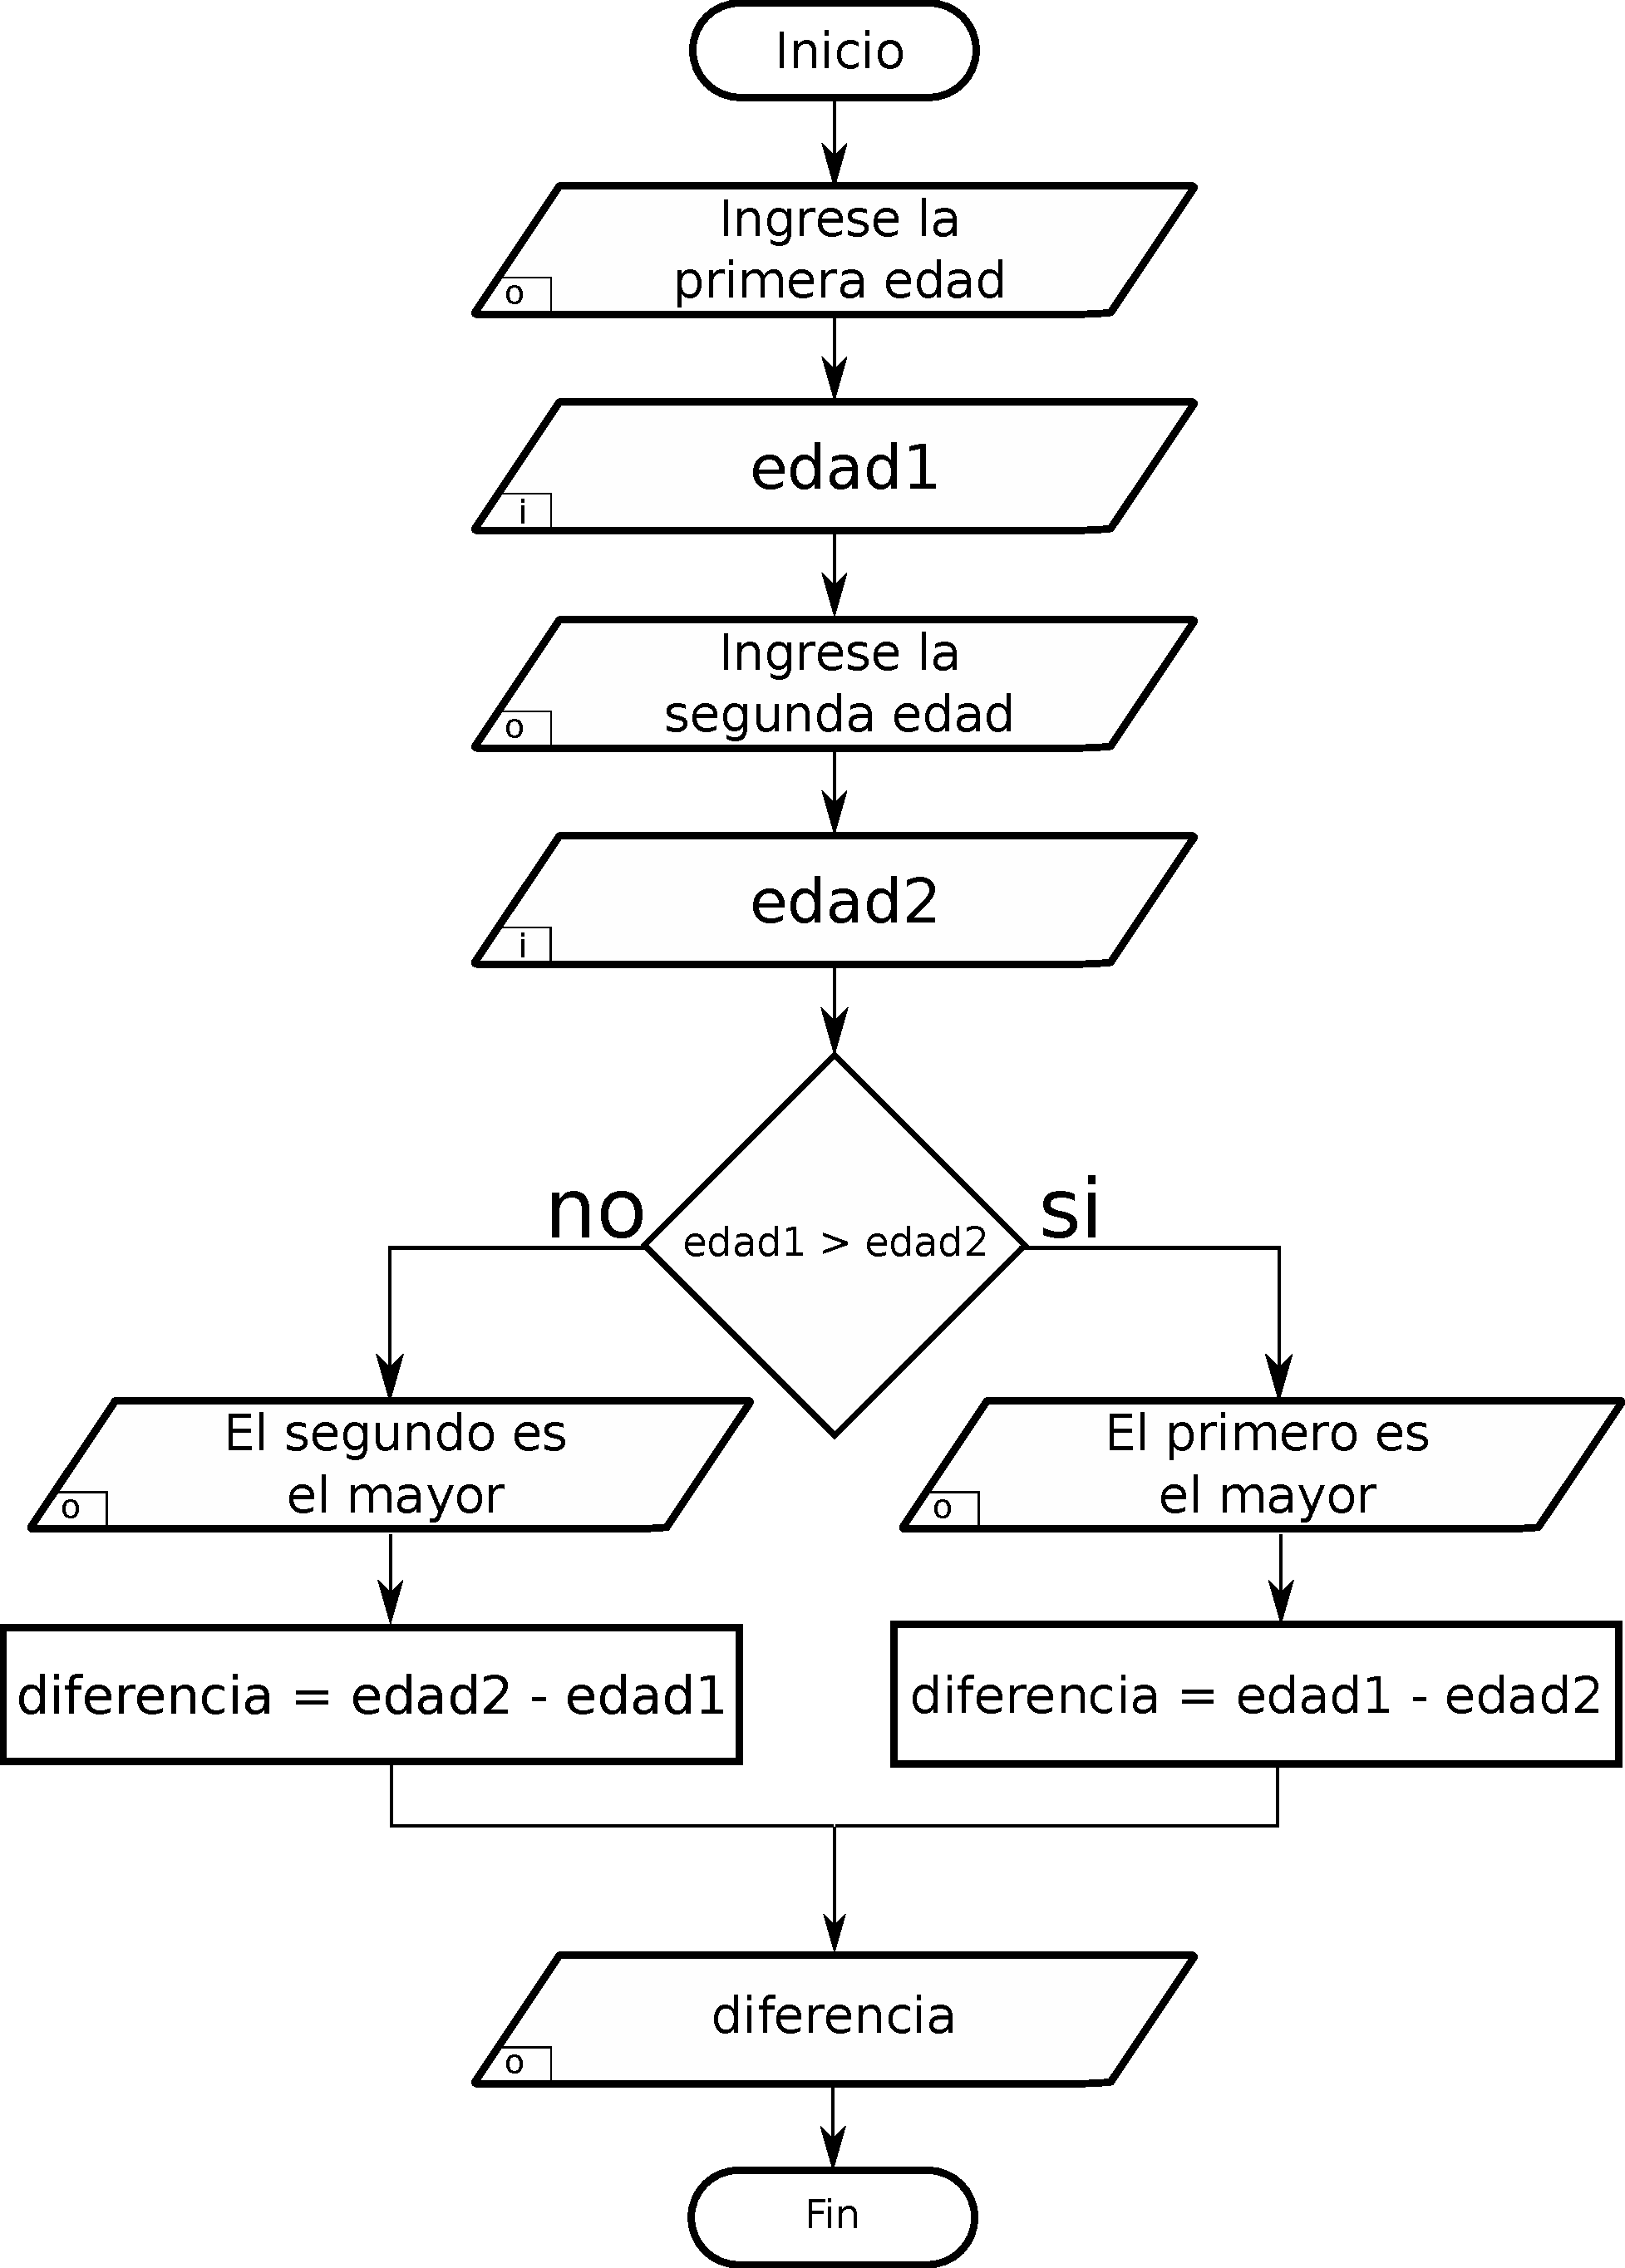
\includegraphics[height=150mm]{./img/ejercicio_2.pdf} 
\end{figure}

\pagebreak

\subsubsection{Ejercicio}
Escribir un algoritmo que imprima los números enteros desde el 0 hasta $N$. Donde el número $N$ es ingresado por el usuario.

\begin{lstlisting}[style=pseudocodigo]
imprimir: Ingrese N
leer: cantidad
para contador desde 0 hasta cantidad hacer
imprimir: contador
fin para
\end{lstlisting}

\begin{figure}[h!]
  \centering
  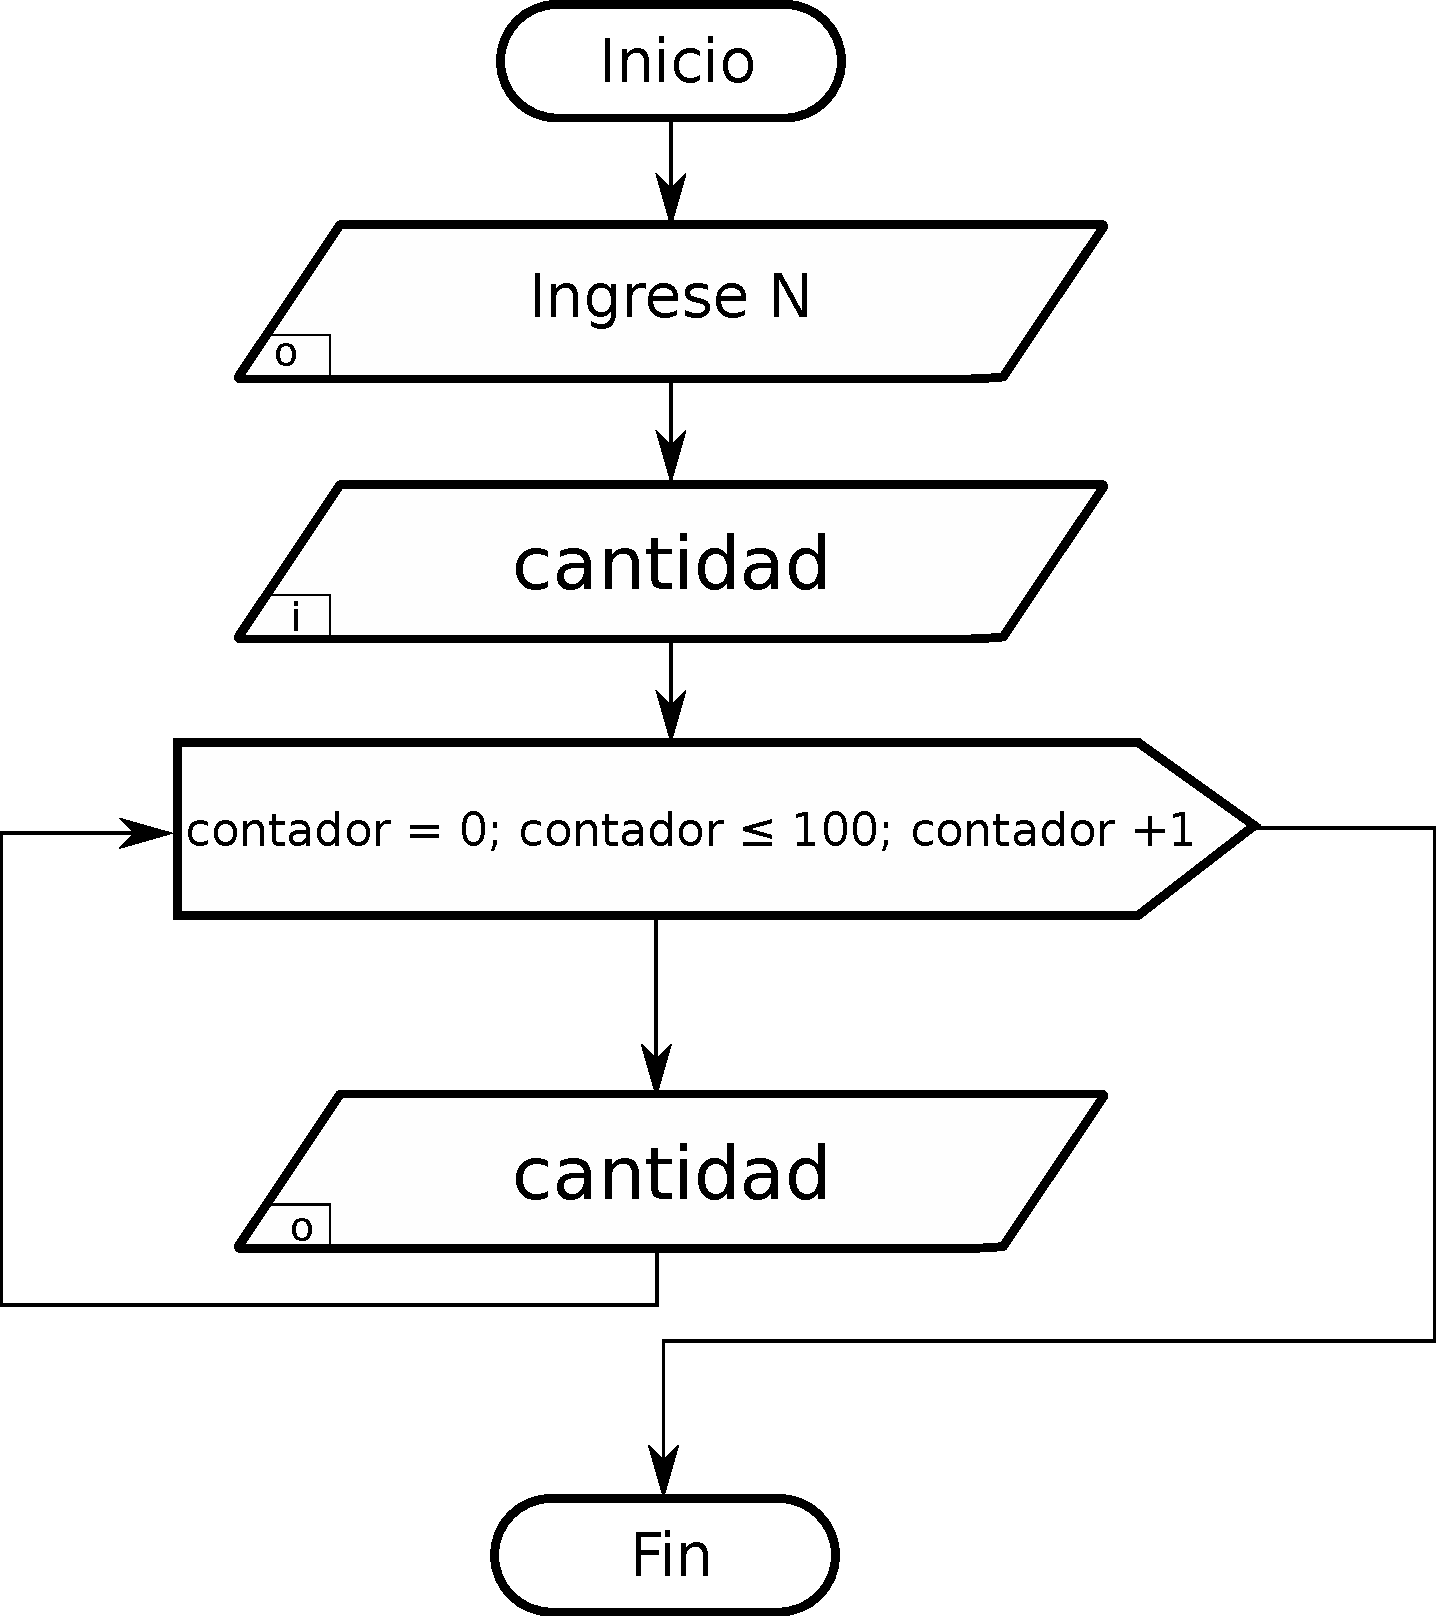
\includegraphics[height=110mm]{./img/ejercicio_3.pdf} 
  \caption{ejercicio 2 versión con bloque \textbf{para}}
\end{figure}

\pagebreak
\subsubsection{Preguntas:}
Completar los espacios en blanco:\\
\begin{enumerate}[a)]
  \item Todos los programas pueden ser escritos en términos de 3 secuencias de control:\underspace,\underspace,\underspace.
  \item La secuencia de control \underspace es utilizada para ejecutar una acción cuando es verdadera y otra acción cuando es falsa.
  \item La secuencia \underspace especifica que una o varias sentencias se ejecutarán repetidamente, mientras la condición sea verdadera.
\end{enumerate}


\pagebreak
% \subsubsection*{Selección}
\subsubsection{Ejercicio}
Escribir un algoritmo para calcular la distancia recorrida (m) por un móvil que se desplaza con velocidad constante (m/s) durante un tiempo (s). 
La velocidad y el tiempo serán ingresadas por el usuario.

\subsubsection{Ejercicio}
Escribir un algoritmo para obtener el promedio simple de un estudiante a partir de las tres notas parciales.
Las notas serán introducidas una a una por el usuario.

\subsubsection{Ejercicio}
En un local se hace un descuento del \%20 cuando la compra supera los \$ 1000. Escribir un algoritmo que calcule el precio a pagar por el cliente
teniendo como dato el valor de la compra.

\subsubsection{Ejercicio}
Escribir un algoritmo que determine si un número $n$ tiene tres cifras. El usuario debe ingresar el número $n$.

\subsubsection{Ejercicio 7}
Escribir un algoritmo que solicite ingresar dos números $n1$ y $n2$. Si el primero es mayor que el segundo mostrar la suma de ambos, por otro lado si el segundo es mayor al primero, mostrar el producto entre los números. En caso de que sean iguales imprimir ``Los números son iguales''.

% \subsubsection{Repetición}
\subsubsection{Ejercicio 8}
Escribir un programa que calcule la potencia $x={num1}^{num2}$, donde $num1$ y $num2$ son números enteros positivos ingresados por el usuario.

\subsubsection{Ejercicio 9}
Escribir un programa que calcule la suma de los primeros \textbf{n} números. El número \textbf{n} es un entero positivo, ingresado por el usuario.

\subsubsection{Ejercicio 10}
Escribir un algoritmo que imprima los número impares desde 0 hasta $N$. Donde $N$ es ingresado por el usuario.

\subsubsection{Ejercicio 11}
Escribir un algoritmo que determine la temperatura promedio de $N$ mediciones de temperatura. El usuario debe ingresar la cantidad $N$ y las $N$ mediciones. 

\subsubsection{Ejercicio 12}
Escribir un algoritmo que determine el mayor de 10 números ingresados. El usuario debe ingresar cada uno de los 10 números.

\subsubsection{Ejercicio 13}
Escribir un algoritmo que determine el mayor de $N$ números positivos ingresados. El usuario debe ingresar cada uno de los $N$ números. Para terminar se debe ingresar un -1.

\subsubsection{Ejercicio 14}
Escribir un algoritmo que solicite ingresar $N$ calificaciones de alumnos y determine la cantidad de aprobados, desaprobados y promocionados. 
El usuario debe ingresar el número $N$ y las $N$ calificaciones.

\underline{Según:}
\begin{itemize}
  \item Desaprobado: nota menor a 6
  \item Aprobado: nota mayor o igual a 6
  \item Promocionado: nota mayor o igual a 8
\end{itemize}

\subsubsection{Ejercicio 15}
Escribir de cuatro formas diferentes, sentencias en C que incrementen en 1 una variable \texttt{X}.
